\documentclass{report}
\usepackage{fullpage}
\usepackage[backend=biber]{biblatex} 
\addbibresource{bibliography.bib}
\usepackage{hyperref}
\hypersetup{
	pdfborderstyle={/S/U/W 1}
}

\usepackage{amsmath}
\usepackage{amssymb}
\usepackage{float}
\usepackage{tikz}
\usepackage{pgfplots}
\usepackage{xcolor}

\begin{document}
	\title{CAB420 Project Report \\ \large{Movie Rating Prediction}}
	\author{
		Jarrod Williams\\
		\texttt{n9722068}\\
		\emph{\dots\%}
		\and 
		Caleb Geizer\\
		\texttt{n9488243}\\
		\emph{\dots\%}
		\and
		Alex Barnier\\
		\texttt{n9448551}\\
		\emph{\dots\%}
		\and	
		Madeline Miller\\
		\texttt{n9342401}\\
		\emph{\dots\%}
	}
	\date{June, 2018}
	\maketitle
	
	\chapter{Introduction}
	\section{Motivations}
	As businesses strive to increase user interaction with their products and services, recommendation systems have seen widespread adoption. One such business is Netflix, arguably the largest platform for watching and rating movies, who uses recommendation systems to provide it’s users with movies it believes are relevant to their tastes. This is achieved by training its recommender system on millions of user reviews. In 2009 Netflix issued a challenge to the community to design a recommendation algorithm that was better than their algorithm at the time. This challenge, called the ‘Netflix Prize’, aimed to create an algorithm with a Root-Mean-Squared-Error (RMSE) of 90\% of their existing one or better.
	
	The motivation for this project was to develop our own solution for this challenge and help better the performance of movie recommendation algorithms. The Netflix Prize winner was announced in 2011 and had a RMSE of 0.8567 \autocite{NeflixLeader}. It is our goal to build a recommender system with a RMSE within the top ten teams, (i.e. RMSE $\leq$ 0.8624).
	\section{Related Work}
	A common approach to creating a recommendation system using this data is using a k-means clustering algorithm to group different users together based on their preferences. This method is used to create larger sample sizes for ratings by treating one cluster as a single user \autocite{CS229}.
	These clusters can then be used in conjunction with a classifier, like naive bayes, to create the final recommendation system. By using a naive bayes classifier features like genre of specific movies or other metadata can be added as a feature to create more refined probabilities. This can also be applied to a multi-class logistic regression classifier \autocite{Bystrom}, where certain features can be given weights, which would allow for place importance on certain genres or directors (if present).
	
	How do we extend these approaches?
	The objectives of this report are to extend the existing approaches put forward by Huang and Bystr\"om to get a classifier close to, or less than the the Netflix Prize’s qualification RMSE of 0.8572 \cite{NeflixRules}.
	
	\chapter{Experiment}
	\section{MovieLens Data}
	\subsection{The Dataset}
	The MovieLens data set consists of approximately 100,000 user ratings for films of various genres and release dates. Each rating is out of 5, representing the ‘star-ratings’ users have assigned to the film. Partial star ratings (e.g. 2.5 stars) are also given, allowing for a total of 10 possible ratings (0.5 - 5 stars). Included with each rating is the film id which links to another table containing the film’s title, genre(s) and release date. As one of the features of the MovieLens website is the ability to add tags to films, the dataset also contains a list of user-defined tags for the movies. Finally, there is a table that links the MovieLens id’s for films to their corresponding id on other community sites like IMDb (Internet Movie Database) and TMDb (The Movie Database). Combined, these tables represent 9125 movies, 100004 user-ratings from 671 users and 1296 custom tags from 61 users.
	\subsection{Pre-processing}
	The data was filtered into only the relevant parts, i.e. only the user id, the rating, the movie id, and the genres of that movie. The headers of the columns were extracted as well for the construction of the pandas dataframes used to store this data. As the genres were provides as a list per movie, they were split up into multiple rows. As an example, the movie ‘Alien’ with the genres Horror and Action, had a row for both the Horror and Action genre.
	
	\subsection{Test and Training Split}
	The data was split into 4 25\%,75\%, test-train splits using an inbuilt function in sklearn, \emph{KFold()}.
	\section{Methedology}
	Three classification algorithms were used for this project: SVM, Random Forest and Gradient Boosting. For all algorithms, the target variable was set to rating with the userId, movieId and genre features used for training and prediction.
	\subsection{SVM Classifier}
	Support Vector Machines (SVM) are a robust and accurate machine learning algorithm designed for classification problems. Originally designed for binary classification, modern SVMs are capable of multiclass classification, regression, ranking and time series prediction \autocite{KarlPersson}. Support vector machines work by separating data using a linear line or hyperplane; separating nonlinear data requires the use of kernel tricks.
	\subsection{Random Forest Classifier}
	\subsection{Gradient Boosting Classifier}
	\section{Parameter Optimisation}
	In order to find which of these algorithms with all of the different parameters was the most efficient, we used parameter optimisation. This involved testing the root mean square error of a set of possible parameters for each algorithm. By iterating through all of the possible combinations, and finding the lowest error, we were able to determine which was the best set of parameters for usage in our model.
	
	Using parameter optimisation is not without its downsides however, as this can introduce overfitting to the test data. In order to get around this, we’ve used cross validation on 4 different splits of data and tested against the mean of the resulting root mean squared error. This allows us to be sure that the parameters work for a wider range of test data than just a single set.
	
	\chapter{Results}
	\section{Comparison to Existing Methods}
	\begin{table}[H]
		\centering
	\begin{tabular}{ccc}
		\hline
		Algorithm & RMSE & \% Improvement\\
		\hline
		K-Means w/ Logistic & 0.884 & \dots	\\
		K-Means w/ Na\"ive Bayes & $>1$ & \dots\\
		Netflix Prize Winner & 0.8567 & 10.06\\
		\hline
	\end{tabular}
	\caption{Comparision of Existing Methods}
	\label{tab:pastresults}
	\end{table}
	\begin{table}[H]
		\centering
		\begin{tabular}{ccc}
			\hline
			Algorithm & RMSE & \% Improvement\\
			\hline
			SVM & $\infty$ & \dots	\\
			Random Forest & 1.091 & \dots\\
			Gradient Boosting & 0.8626 & 9.7\\
			\hline
		\end{tabular}
	\caption{Comparison of Our Results}
	\label{tab:ourresults}
	\end{table}
	\section{Discussion}
	Results show that out of all the approaches we have taken, the Gradient Boosting classifier has the best result with an average RMSE value of 0.8598. The Random Forest classifier tested gives an RMSE value of 1.091. When compared with other classifiers, the Gradient Boosting performs well with a 9.7\% improvement from netflix’ baseline of 0.9525. It also comes close to the Netflix Prize Winner of 0.8567.
%	\begin{figure}[H]
%		\centering
%		\begin{tikzpicture}
%			\begin{axis}[xbar stacked,
%			symbolic y coords={SVM,Random Forest,Gradient Boosting},
%			ytick=data]
%				\addplot[xbar,fill=blue] coordinates {
%					(0,SVM)
%					(1.091,Random Forest)
%					(0.8,Gradient Boosting)
%				};
%				%\addplot[no marks] coordinates {(0.9525,SVM) (0.9525,Gradient Boosting)};
%				\draw[ultra thin, red] (axis cs:0.9525,SVM) -- (axis cs:0.9525,{Gradient Boosting}) node[pos=0.03, below] {Cinematch};
%			\end{axis}
%		\end{tikzpicture}
%		\caption{Chart of Our Classifiers in Relation to Cinematch Baseline}
%		\label{fig:graphofours}
%	\end{figure}
	
	\begin{figure}[H]
		\centering
		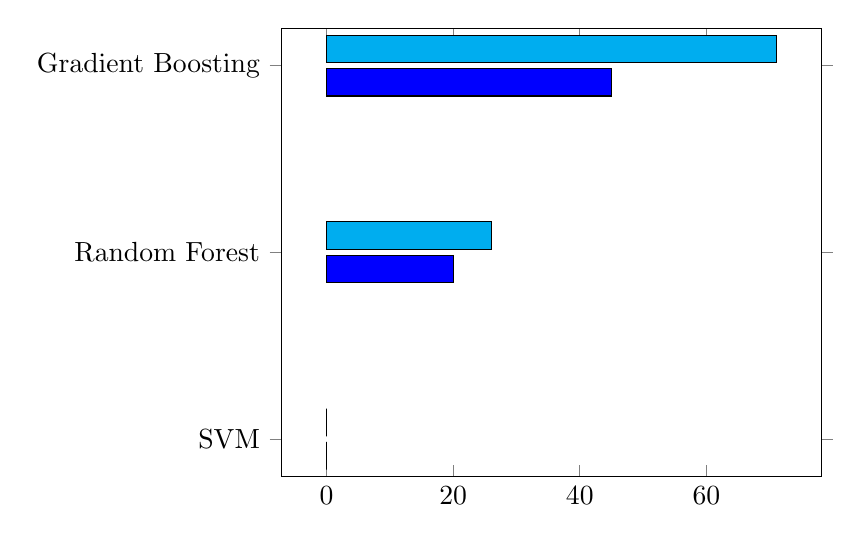
\begin{tikzpicture}
			\begin{axis}[xbar,
						symbolic y coords={SVM,Random Forest,Gradient Boosting},
						ytick=data]
			\addplot[xbar,fill=blue] coordinates {
					(0,SVM)
					(20,Random Forest)
					(45,Gradient Boosting)
			};
			\addplot[xbar,fill=cyan] coordinates {
				(0,SVM)
				(26,Random Forest)
				(71,Gradient Boosting)
			};
			\end{axis}
		\end{tikzpicture}
		\caption{Chart of Our Classifier Accuracy}
		\label{fig:graphofours}
	\end{figure}
	
	When comparing the accuracy percentage, Gradient Boosting gives a much better result in both the initial and optimised algorithms. Gradient Boosting shows an initial accuracy of $\approx45\%$ and a final accuracy of 71\% when optimised.
	
	\chapter{Conclusion}
	The experiments conducted in this report show that the Gradient Boosting classifier completes the objective of developing an effective movie rating prediction algorithm. The Root-Mean-Squared-Error of 0.8598 places the algorithm in the top 10 algorithms in the Netflix Prize contest.
	
	A shortcoming of our approach was that the dataset used was designed to easily develop these types of recommendation algorithms. Therefore, there was no bad data in the dataset that might reduce the accuracy of the results. If the dataset used had these bad data points, the algorithms might give a different result.
	
	\newpage
	\printbibliography
	
\end{document}